\clearpage
\section{Результаты}

\subsection{Анализ всех найденных видов}

Были проанализированы 413 нуклеотидных последовательностей гена \textit{Nxf1} у представителей различных филогенетических групп из клад Cnidaria (Стрекающие) и Bilateria (Двусторонне-симметричные).
Организмы, относящиеся к Mammalia, в анализ не были взяты в связи с уже имеющимися для них данными.


Для таксономических групп более низкого ранга с небольшим количеством видов в них с помощью PSI-BLAST были увеличены выборки, где это оказалось возможным, результат продемонстрирован на таблице~\ref{tab:psi_blast}.

\begin{longtable}[c]{|c|c|c|c|c|}
\caption{Результат увеличения выборки с помощью PSI-BLAST.}
\label{tab:psi_blast}\\
\hline
\textbf{\begin{tabular}[c]{@{}c@{}}Филогенетическая\\ группа\end{tabular}} &
  \textbf{\begin{tabular}[c]{@{}c@{}}Таксон\\ высокого\\ ранга\end{tabular}} &
  \textbf{\begin{tabular}[c]{@{}c@{}}Видов до\\ PSI-BLAST\end{tabular}} &
  \textbf{\begin{tabular}[c]{@{}c@{}}Видов\\ добавлено\end{tabular}} &
  \textbf{\begin{tabular}[c]{@{}c@{}}Итого\\ видов\end{tabular}} \\ \hline
\endfirsthead
%
\endhead
%
\multirow{2}{*}{\begin{tabular}[c]{@{}c@{}}Bilateria→Protostomia\end{tabular}} & Ecdysozoa & 56 & 42 & 98 \\
                                                                                  & Spiralia  & 6  & 63 & 69 \\ \hline
Cnidaria                                                                          & Anthozoa  & 2  & 12 & 14 \\ \hline
\end{longtable}

В итоге для 353 видов удалось найти ``консервативную кассету`` и продолжить дальнейший анализ.


На рисунке~\ref{fig:tree_summary} отображено распределение исследованных видов по таксонам высокого ранга.
Последовательно идущие таксоны объединены в один блок и разделены пунктиром.

\begin{figure}[h] % here, top, bottom, page
    \centering
    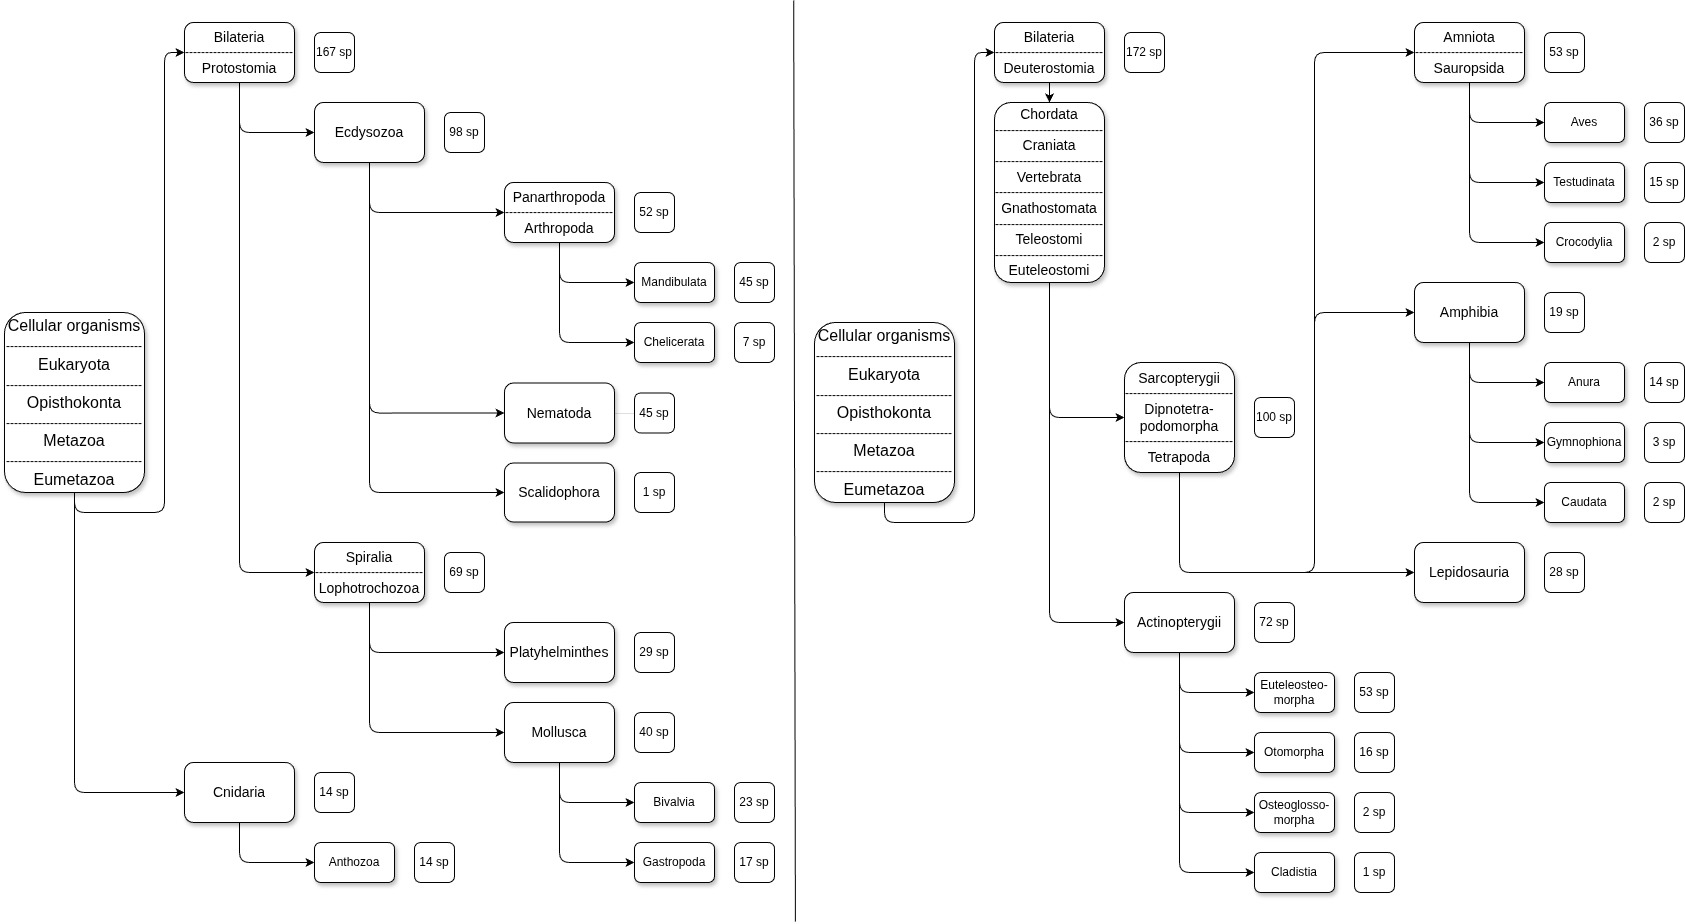
\includegraphics[width=1.0\textwidth]{images/Tree_summary}
    \caption{Количество видов, взятых в анализ, для разных таксономических групп.}
    \label{fig:tree_summary}
\end{figure}

В таблице~\ref{tab:Comparison_groups} можно ознакомиться с некоторыми характеристиками ``консервативной кассеты`` для всех исследованных групп.

Для всех видов, имеющих ``кассету``, были построены вторичные структуры для интрон-содержащего транскрипта с выделением цветом ``кассетного`` интрона.


\begin{longtable}[c]{|c|c|c|c|c|c|}
\caption{Характеристики ``консервативной кассеты`` для всех исследованных групп.}
\label{tab:Comparison_groups}\\
\hline
\textbf{\begin{tabular}[c]{@{}c@{}}Название\\ таксона\end{tabular}} &
  \textbf{\begin{tabular}[c]{@{}c@{}}Стат.\\ метрики\end{tabular}} &
  \textbf{\begin{tabular}[c]{@{}c@{}}Кол-во\\ нуклеотидов\\ до стоп-кодона\\ в интроне\end{tabular}} &
  \textbf{\begin{tabular}[c]{@{}c@{}}Длина\\ 1-го экзона\\ в кассете\end{tabular}} &
  \textbf{\begin{tabular}[c]{@{}c@{}}Длина\\ кассетного\\ интрона\end{tabular}} &
  \textbf{\begin{tabular}[c]{@{}c@{}}Длина\\ 2-го экзона\\ в кассете\end{tabular}} \\ \hline
\endfirsthead
%
\endhead
%
\hline
\endfoot
%
\endlastfoot
%
\multirow{3}{*}{\begin{tabular}[c]{@{}c@{}}Ecdysozoa,\\ 98 видов\end{tabular}}     & Min    & 1                  & 83                   & 47    & \multirow{3}{*}{37} \\
                                                                                   & Median & 22                 & 110                  & 375   &                     \\
                                                                                   & Max    & 1345               & 307                  & 9821  &                     \\ \hline
\multirow{3}{*}{\begin{tabular}[c]{@{}c@{}}Spiralia,\\ 69 видов\end{tabular}}      & Min    & 1                  & 56                   & 222   & \multirow{3}{*}{37} \\
                                                                                   & Median & 1                  & 221                  & 1706  &                     \\
                                                                                   & Max    & 19                 & 242                  & 18219 &                     \\ \hline
\multirow{3}{*}{\begin{tabular}[c]{@{}c@{}}Cnidaria,\\ 14 видов\end{tabular}}      & Min    & 10                 & 86                   & 116   & \multirow{3}{*}{37} \\
                                                                                   & Median & 40                 & 116                  & 531   &                     \\
                                                                                   & Max    & 103                & 116                  & 991   &                     \\ \hline
\multirow{3}{*}{\begin{tabular}[c]{@{}c@{}}Sauropsida,\\ 53 вида\end{tabular}}     & Min    & 1                  & 107                  & 443   & \multirow{3}{*}{37} \\
                                                                                   & Median & 142                & 110                  & 1393  &                     \\
                                                                                   & Max    & 1519               & 110                  & 3942  &                     \\ \hline
\multirow{3}{*}{\begin{tabular}[c]{@{}c@{}}Amphibia,\\ 19 видов\end{tabular}}      & Min    & 1                  & \multirow{3}{*}{110} & 2004  & \multirow{3}{*}{37} \\
                                                                                   & Median & 25                 &                      & 3029  &                     \\
                                                                                   & Max    & 187                &                      & 10340 &                     \\ \hline
\multirow{3}{*}{\begin{tabular}[c]{@{}c@{}}Lepidosauria,\\ 28 видов\end{tabular}}  & Min    & \multirow{3}{*}{1} & \multirow{3}{*}{110} & 2293  & \multirow{3}{*}{37} \\
                                                                                   & Median &                    &                      & 2579  &                     \\
                                                                                   & Max    &                    &                      & 4667  &                     \\ \hline
\multirow{3}{*}{\begin{tabular}[c]{@{}c@{}}Actinopterygii,\\ 72 вида\end{tabular}} & Min    & 1                  & \multirow{3}{*}{110} & 1702  & \multirow{3}{*}{37} \\
                                                                                   & Median & 22                 &                      & 2549  &                     \\
                                                                                   & Max    & 283                &                      & 4202  &                     \\ \hline
\end{longtable}


\subsection{Подробный анализ Actinopterygii}

Для таксономической группы Actinopterygii проводился более углубленный анализ, так как на текущий момент данных по гену \textit{Nxf1} для них не было.
Были взяты все найденные нуклеотидные последовательности гена у представители данной филогенетической группы – 72 вида.

В таблице~\ref{tab:Actinopterygii} из приложения показана характеристика ``консервативной кассеты`` исследуемой группы.
Результаты по другим группам можно также найти в приложении, таблицы~\ref{tab:Ecdysozoa}--\ref{tab:Lepidosauria}.

На рисунках~\ref{fig:Actinopterygii_intron} и~\ref{fig:Actinopterygii_intron_stop} показано распределение длин ``кассетного`` интрона и длин части ``кассетного`` интрона до стоп-кодона, соответственно.

\begin{figure}[hb] % here, top, bottom, page
    \centering
    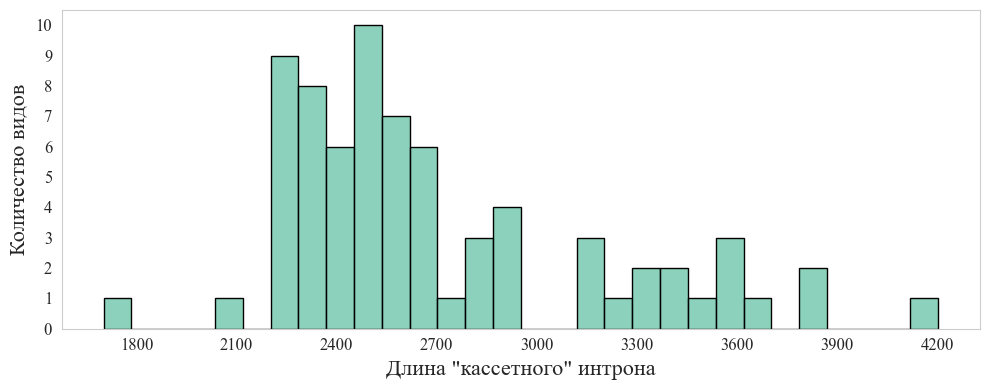
\includegraphics[width=0.75\textwidth]{images/Actinopterygii_intron}
    \caption{Распределение длин ``кассетного`` интрона у Actinopterygii}
    \label{fig:Actinopterygii_intron}
\end{figure}

\begin{figure}[ht] % here, top, bottom, page
    \centering
    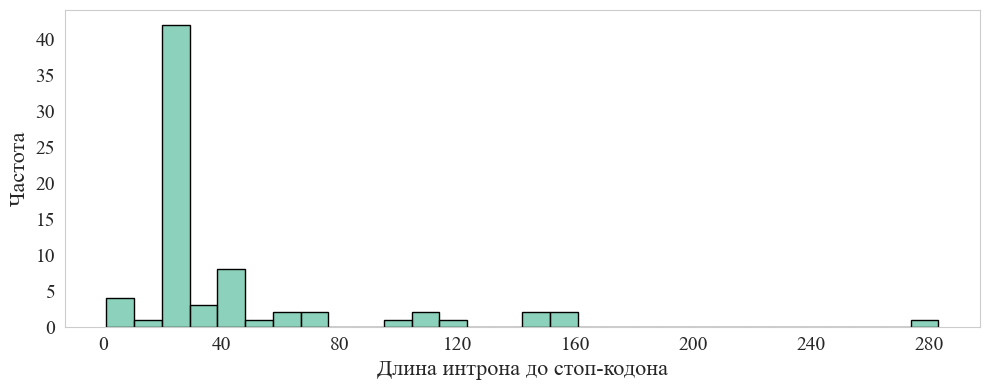
\includegraphics[width=0.75\textwidth]{images/Actinopterygii_intron_stop}
    \caption{Распределение длин части ``кассетного`` интрона до стоп-кодона у Actinopterygii}
    \label{fig:Actinopterygii_intron_stop}
\end{figure}

На рисунке~\ref{fig:Actinopterygii_maxentscan} представлены результаты оценки ``силы сайтов сплайсинга`` - ``ящики с усами``, отображающие распределение MaxEntScan score для таксонов более низкого ранга внутри группы Actinopterygii.
Разбиение на подгруппы основано на их удаленности друг от друга.
Порядок групп на графике не несет смысловой нагрузки.

\begin{figure}[h] % here, top, bottom, page
    \centering
    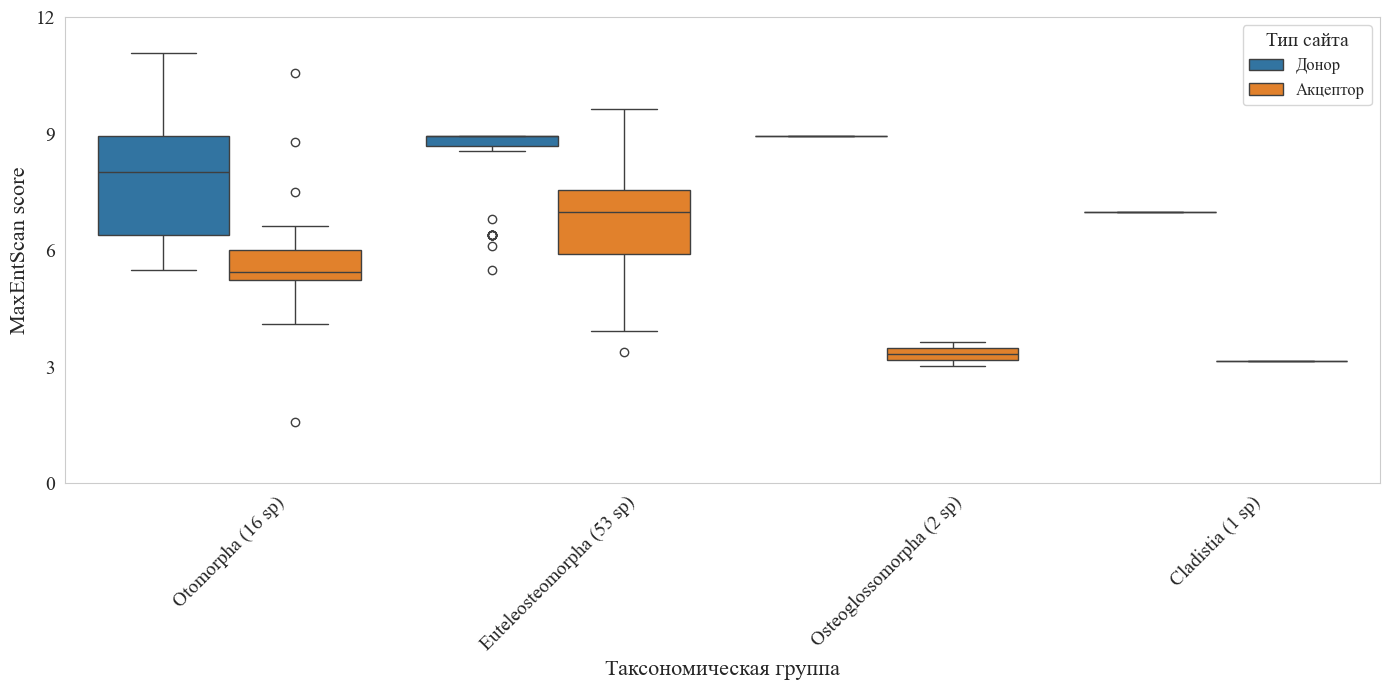
\includegraphics[width=1.0\textwidth]{images/Actinopterygii_maxentscan}
    \caption{Результаты проведения MaxEntScan для Actinopterygii.}
    \label{fig:Actinopterygii_maxentscan}
\end{figure}


Рисунок~\ref{fig:Actinopterygii_meme} демонстрирует результаты, полученные с помощью MEME Suite.

Найденные мотивы присутствуют не у всех видов, взятых в анализ изначально, их количество отображено в столбце Sites.
Нас заинтересовал 2-й найденный мотив, так как его начало схоже с предложенной авторами~\cite{cte_consensus} консенсусной последовательностью для CTE из рисунка~\ref{fig:CTE_consensus}.
К сожалению, использование Tomtom для сравнения найденных консервативных мотивов из ``кассетного`` интрона с базой данных не дало статистически значимых результатов.

\begin{figure}[h] % here, top, bottom, page
    \centering
    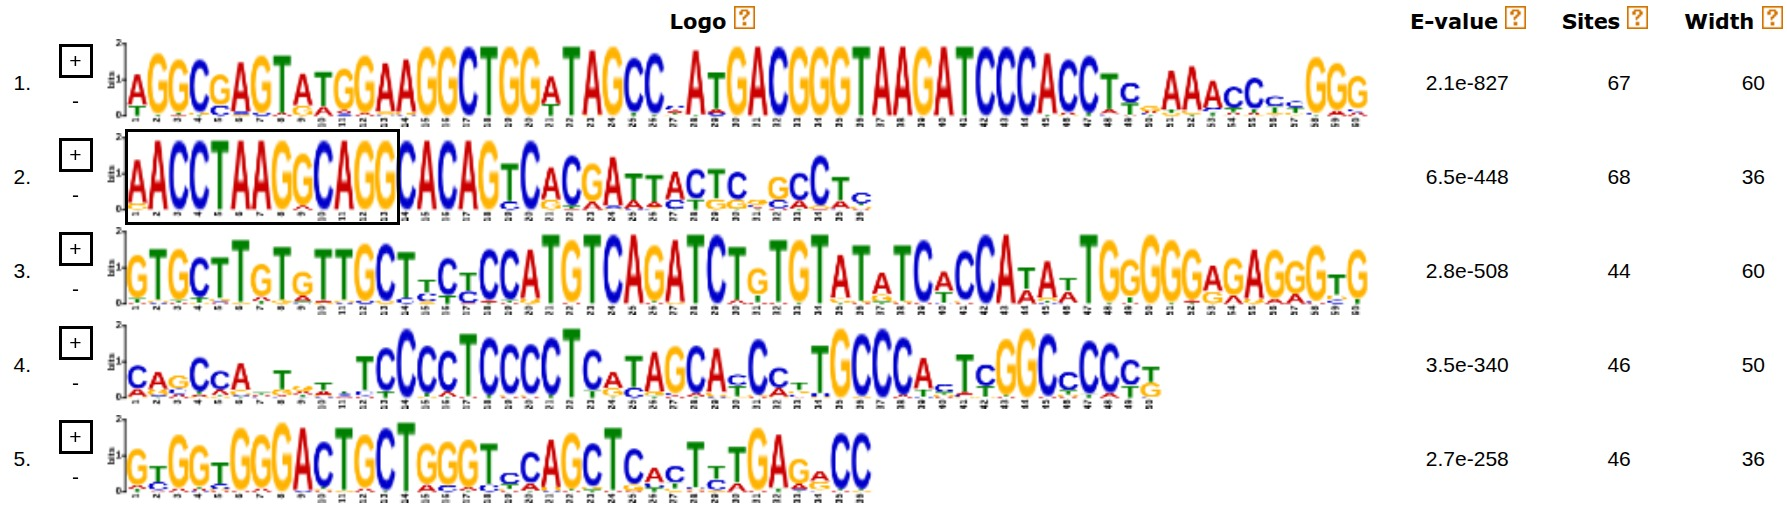
\includegraphics[width=1.0\textwidth]{images/Actinopterygii_meme_motif}
    \caption{Результат поиска мотивов внутри ``кассетного`` интрона с помощью MEME Suite для Actinopterygii. Черным прямоугольником выделен участок, похожий на консенсусную последовательность CTE (рис.~\ref{fig:CTE_consensus})~\cite{cte_consensus}}
    \label{fig:Actinopterygii_meme}
\end{figure}.

\begin{figure}[H] % here, top, bottom, page
    \centering
    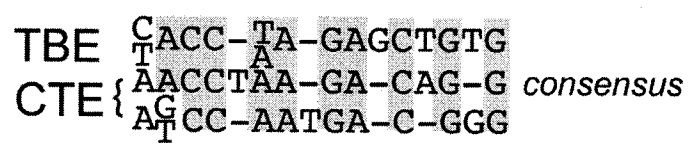
\includegraphics[width=0.7\textwidth]{images/CTE_consensus}
    \caption{Консенсусный конститутивный транспортный элемент (CTE)~\cite{cte_consensus}.}
    \label{fig:CTE_consensus}
\end{figure}

\vspace{1cm}

Репрезентация вторичной структуры интрон-содержащего транскрипта с выделенным кассетным интроном и найденным мотивом показана на рисунке~\ref{fig:Chanos_chanos_2nd_structure}.
У всех видов были сходные структуры и в качестве иллюстрации представлен один из проанализированных видов.

Учитывая тот факт, что мотив с интересующим нас участком, был найден у 68 видов, именно для них был проведен последующий анализ.

Рисунок~\ref{fig:Actinopterygii_alignment_ruler} отображает результаты множественного выравнивания, а на рисунке~\ref{fig:Actinopterygii_tree} представлено филогенетическое дерево, построенное по результатам этого выравнивания.

\begin{sidewaysfigure}
    \centering
    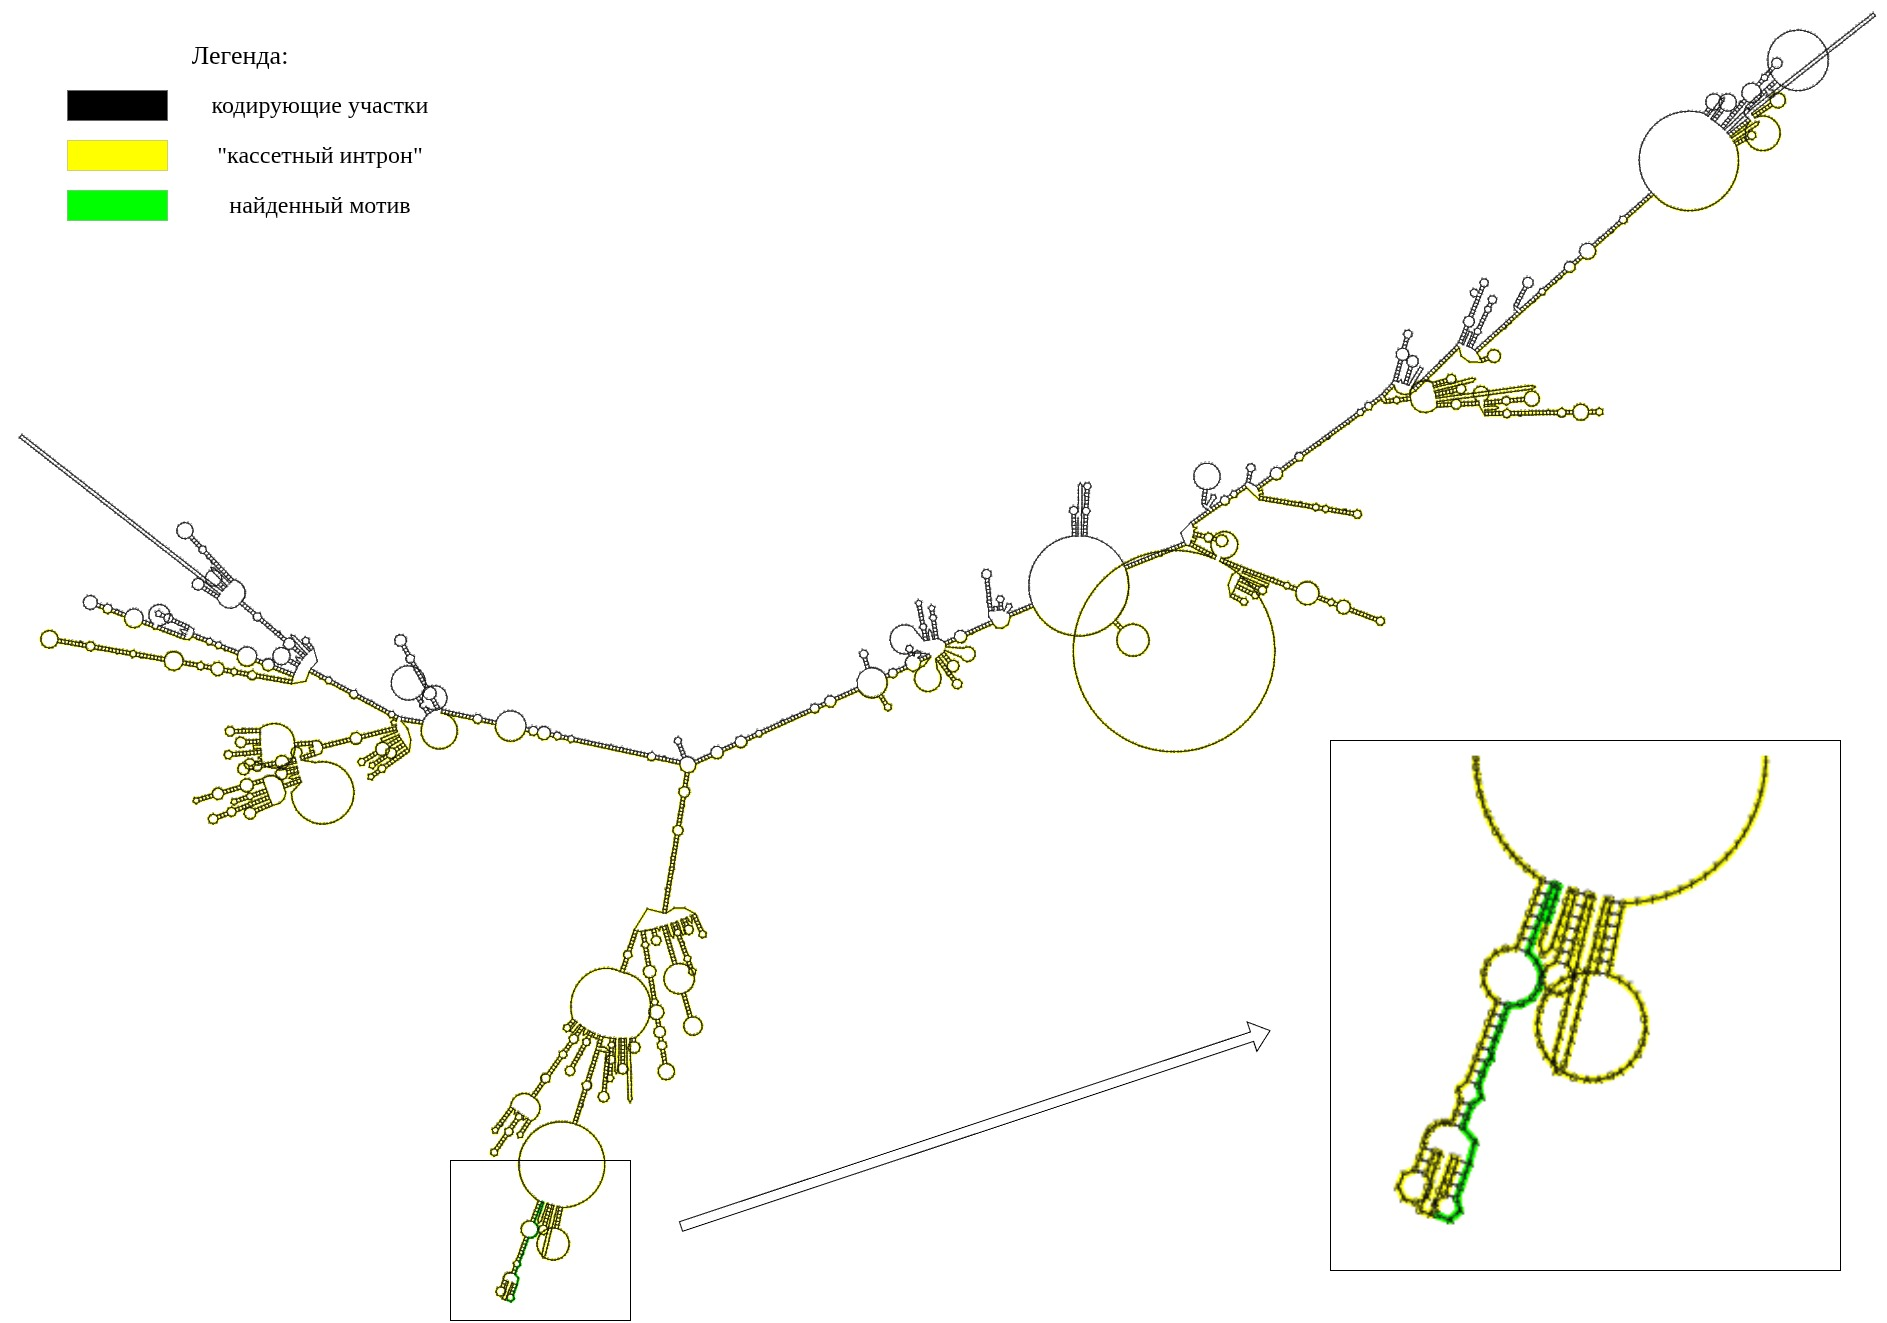
\includegraphics[width=0.9\textheight]{images/Chanos_chanos_2nd_structure}
    \caption{Вторичная структура РНК-транскрипта для \textit{Chanos chanos} из Otomorpha, содержащая ``кассетный`` интрон.}
    \label{fig:Chanos_chanos_2nd_structure}
\end{sidewaysfigure}

\begin{figure}[ht] % here, top, bottom, page
    \centering
    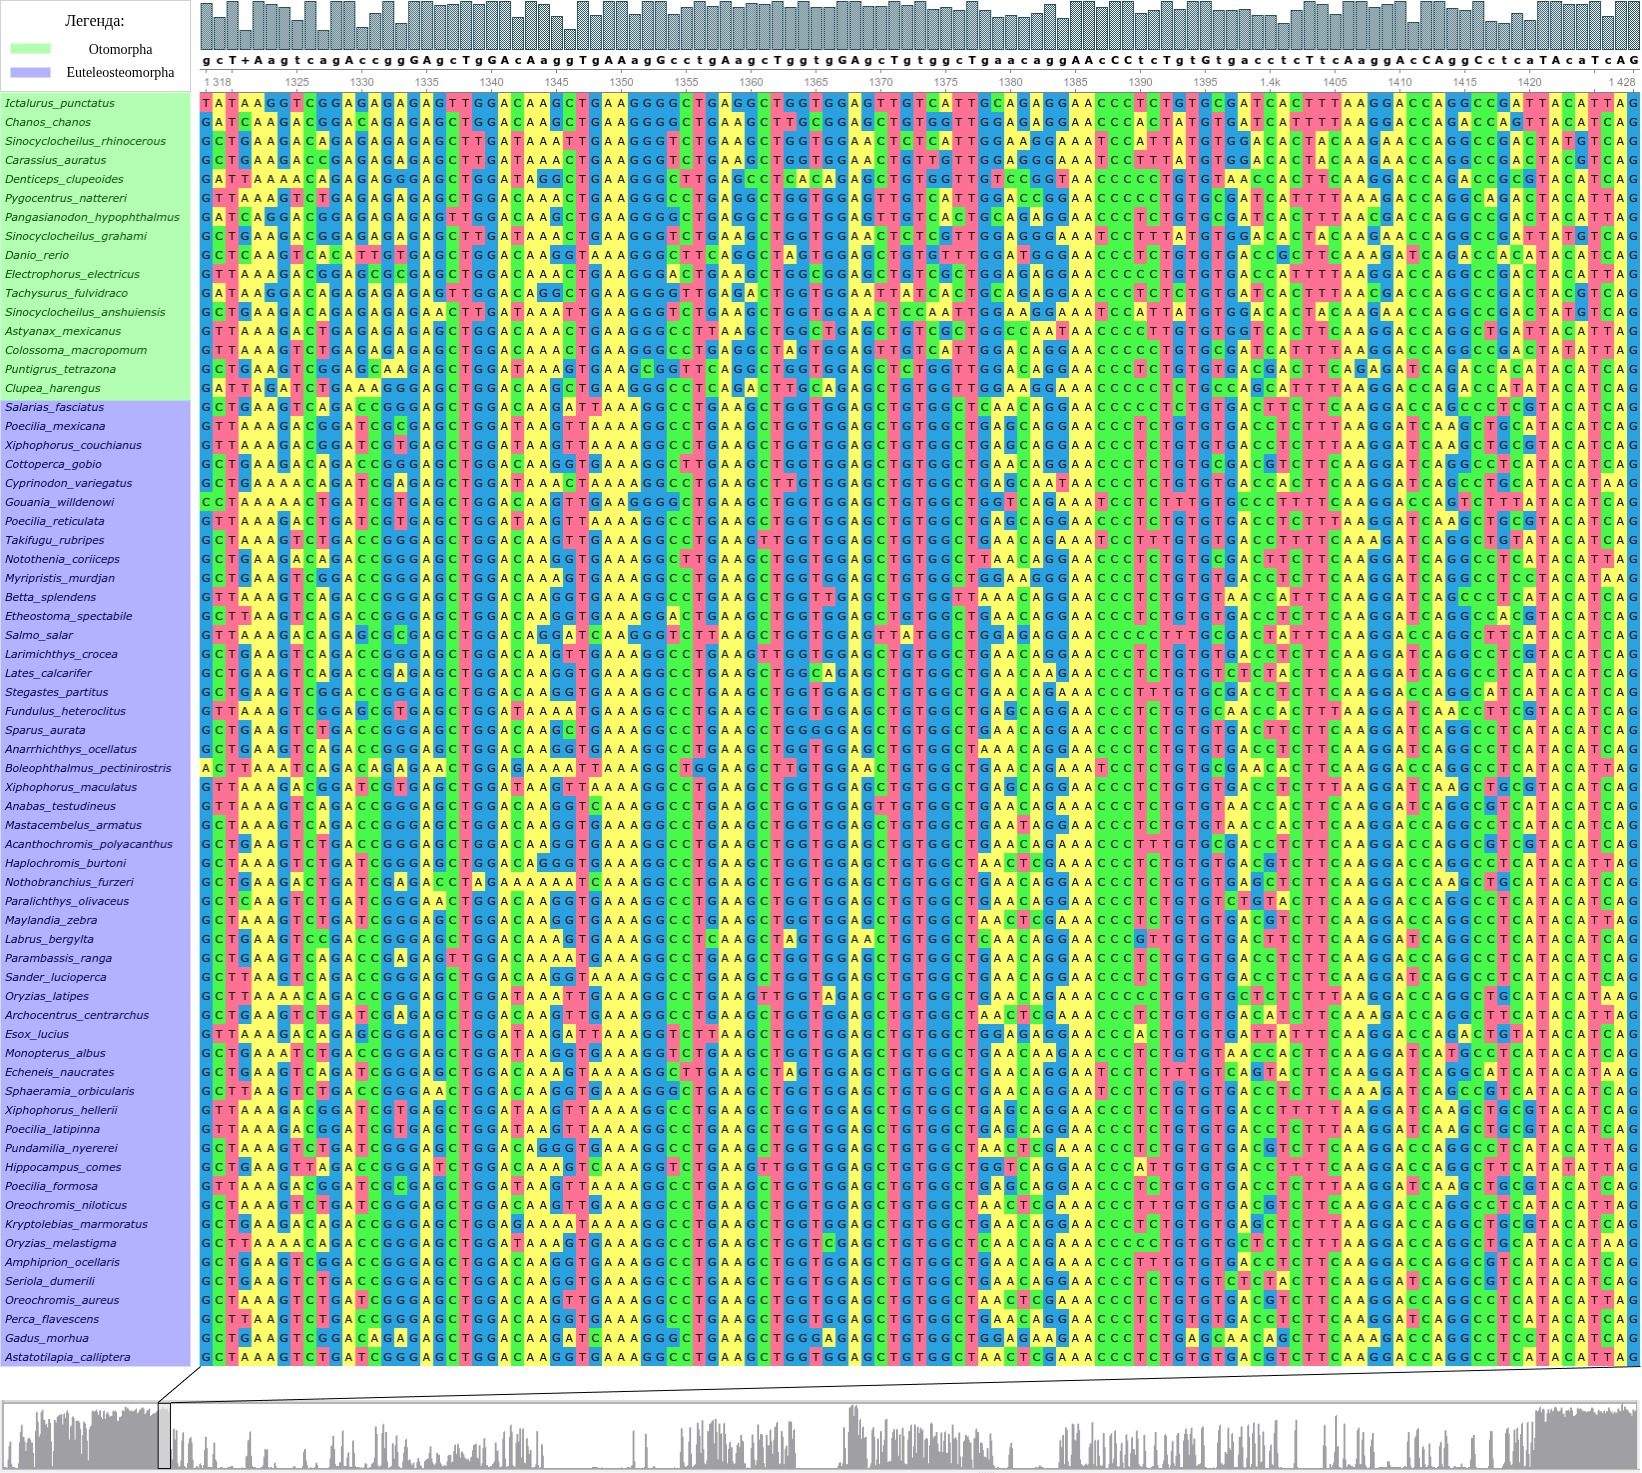
\includegraphics[width=0.9\textwidth]{images/Actinopterygii_alignment_ruler}
    \caption{Результаты множественного выравнивания для Actinopterygii.}
    \label{fig:Actinopterygii_alignment_ruler}
\end{figure}

\begin{figure}[hb] % here, top, bottom, page
    \centering
    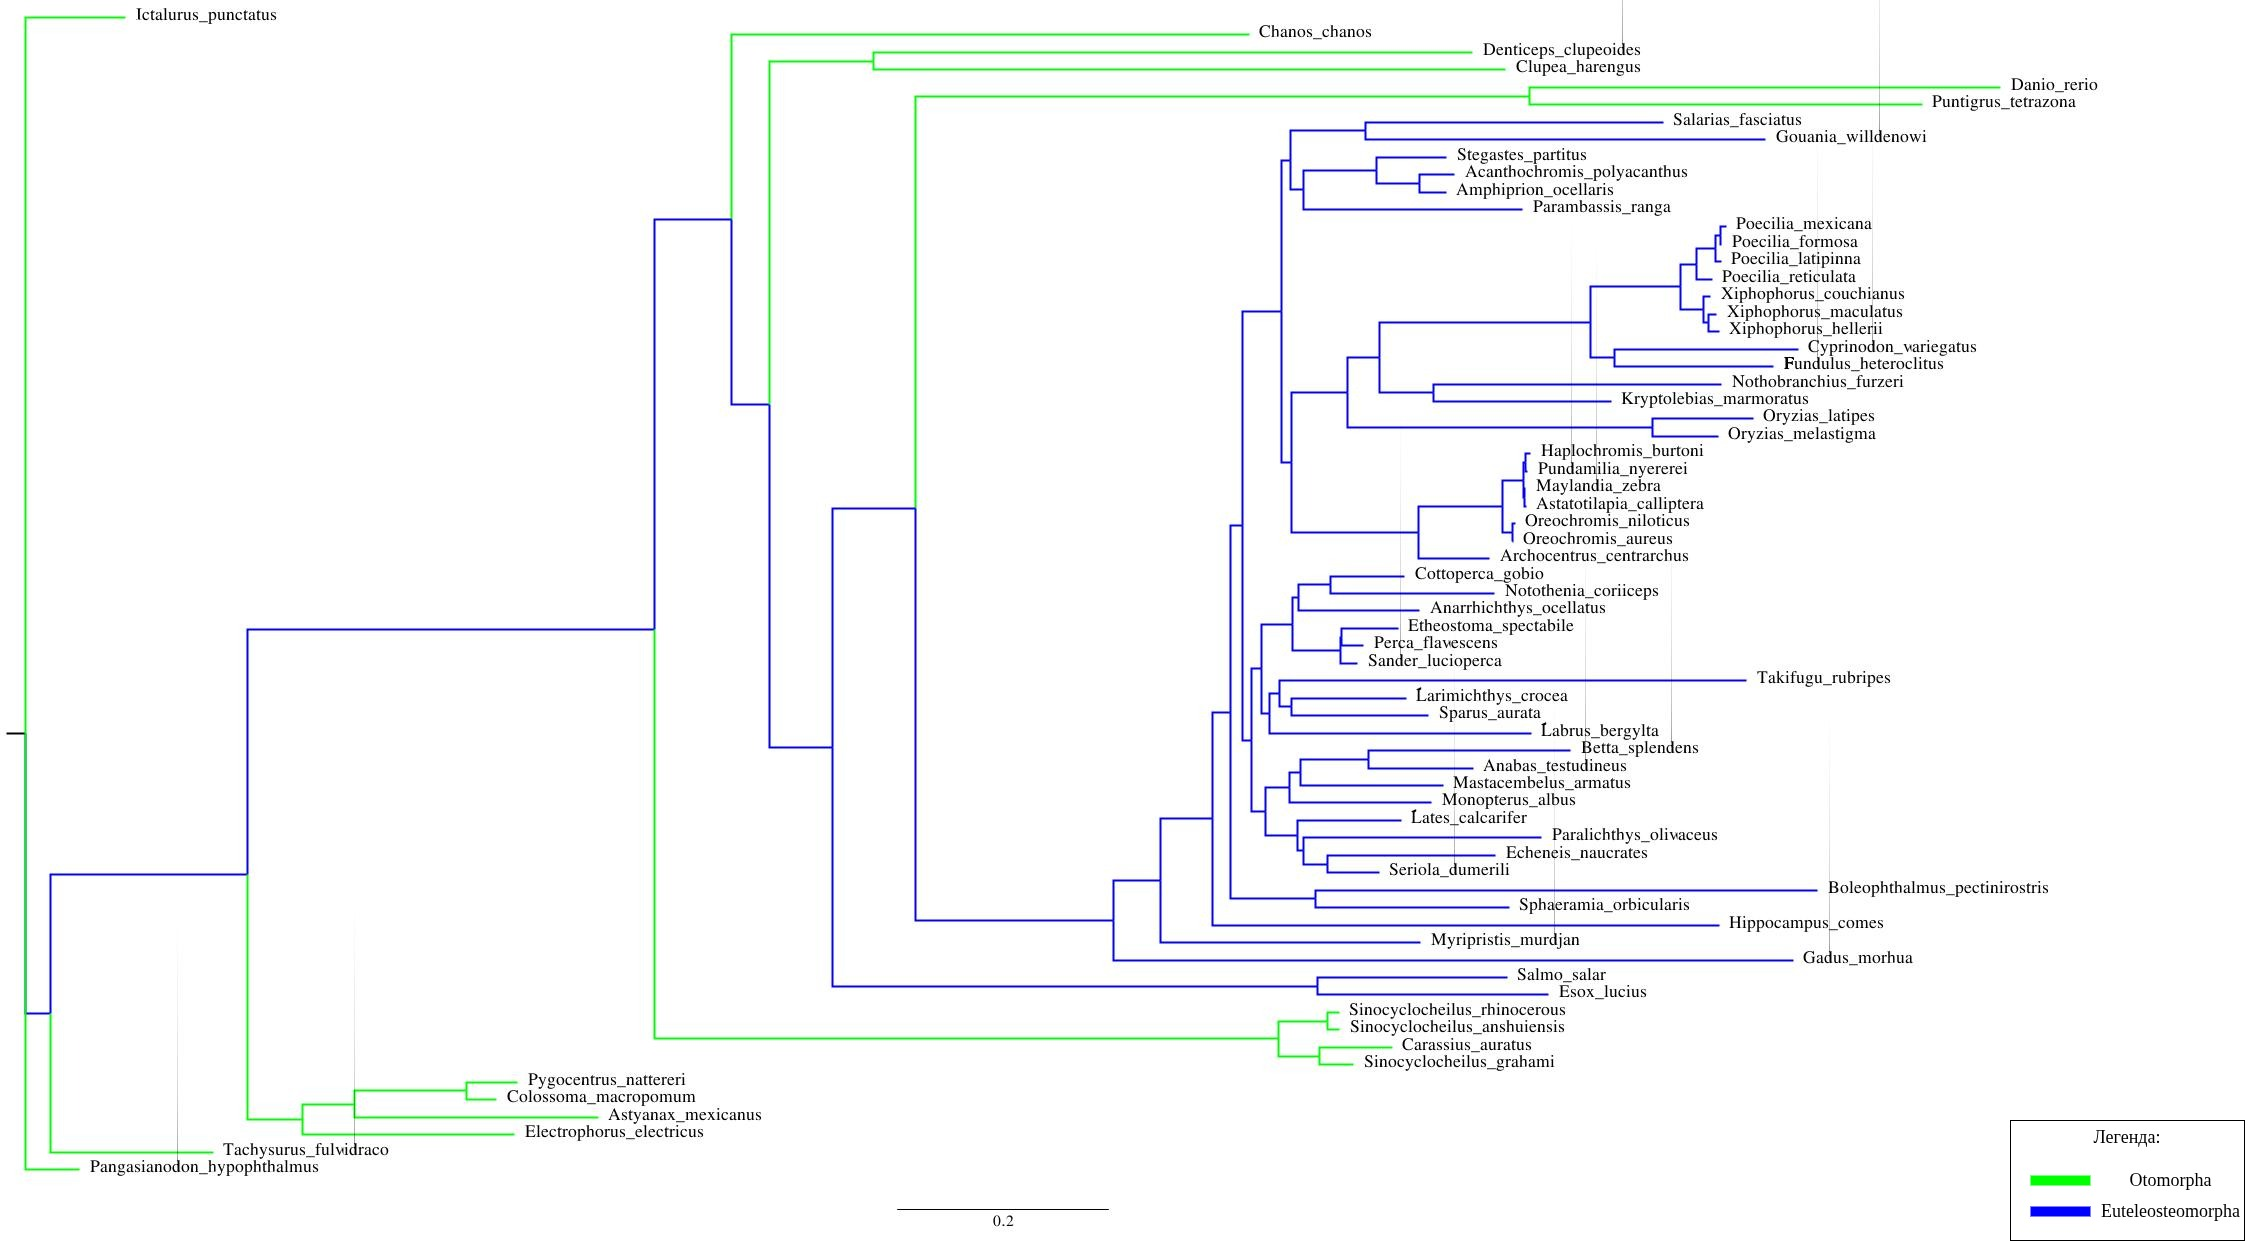
\includegraphics[width=1.0\textwidth]{images/Actinopterygii_tree}
    \caption{Филогенетическое дерево для Actinopterygii.}
    \label{fig:Actinopterygii_tree}
\end{figure}